\documentclass[11pt]{article}

% Change "review" to "final" to generate the final (sometimes called camera-ready) version.
% Change to "preprint" to generate a non-anonymous version with page numbers.
\usepackage[review]{acl}

% Standard package includes
\usepackage{times}
\usepackage{latexsym}

% polyglossia removed — requires XeLaTeX; pdflatex (Overleaf default) is used instead.
% Bengali script examples appear in the supplementary material, not the paper body.

\usepackage{array}
\usepackage{float}
\usepackage{amsmath}

% For proper rendering and hyphenation of words containing Latin characters (including in bib files)
\usepackage[T1]{fontenc}
% For Vietnamese characters
% \usepackage[T5]{fontenc}
% See https://www.latex-project.org/help/documentation/encguide.pdf for other character sets

% This assumes your files are encoded as UTF8
\usepackage[utf8]{inputenc}

% This is not strictly necessary, and may be commented out,
% but it will improve the layout of the manuscript,
% and will typically save some space.
\usepackage{microtype}

% This is also not strictly necessary, and may be commented out.
% However, it will improve the aesthetics of text in
% the typewriter font.
\usepackage{inconsolata}

%Including images in your LaTeX document requires adding
%additional package(s)
\usepackage{graphicx}

% If the title and author information does not fit in the area allocated, uncomment the following
%
%\setlength\titlebox{<dim>}
%
% and set <dim> to something 5cm or larger.

\title{From Words to Images: A Multimodal Benchmark for Bangla Political Stance Detection}

% Author information can be set in various styles:
% For several authors from the same institution:
% \author{Author 1 \and ... \and Author n \\
%         Address line \\ ... \\ Address line}
% if the names do not fit well on one line use
%         Author 1 \\ {\bf Author 2} \\ ... \\ {\bf Author n} \\
% For authors from different institutions:
% \author{Author 1 \\ Address line \\  ... \\ Address line
%         \And  ... \And
%         Author n \\ Address line \\ ... \\ Address line}
% To start a separate ``row'' of authors use \AND, as in
% \author{Author 1 \\ Address line \\  ... \\ Address line
%         \AND
%         Author 2 \\ Address line \\ ... \\ Address line \And
%         Author 3 \\ Address line \\ ... \\ Address line}

\author{Meherunnesa Hossain Ibnath \\
  Ahsanullah University of Science and Technology / Dhaka, Bangladesh\\
  \texttt{meherunnesa.ibnath20@gmail.com} \\\And
  Second Author \\
  Affiliation / Address line 1 \\
  Affiliation / Address line 2 \\
  Affiliation / Address line 3 \\
  \texttt{email@domain} \\}

%\author{
%  \textbf{First Author\textsuperscript{1}},
%  \textbf{Second Author\textsuperscript{1,2}},
%  \textbf{Third T. Author\textsuperscript{1}},
%  \textbf{Fourth Author\textsuperscript{1}},
%\\
%  \textbf{Fifth Author\textsuperscript{1,2}},
%  \textbf{Sixth Author\textsuperscript{1}},
%  \textbf{Seventh Author\textsuperscript{1}},
%  \textbf{Eighth Author \textsuperscript{1,2,3,4}},
%\\
%  \textbf{Ninth Author\textsuperscript{1}},
%  \textbf{Tenth Author\textsuperscript{1}},
%  \textbf{Eleventh E. Author\textsuperscript{1,2,3,4,5}},
%  \textbf{Twelfth Author\textsuperscript{1}},
%\\
%  \textbf{Thirteenth Author\textsuperscript{3}},
%  \textbf{Fourteenth F. Author\textsuperscript{2,4}},
%  \textbf{Fifteenth Author\textsuperscript{1}},
%  \textbf{Sixteenth Author\textsuperscript{1}},
%\\
%  \textbf{Seventeenth S. Author\textsuperscript{4,5}},
%  \textbf{Eighteenth Author\textsuperscript{3,4}},
%  \textbf{Nineteenth N. Author\textsuperscript{2,5}},
%  \textbf{Twentieth Author\textsuperscript{1}}
%\\
%\\
%  \textsuperscript{1}Affiliation 1,
%  \textsuperscript{2}Affiliation 2,
%  \textsuperscript{3}Affiliation 3,
%  \textsuperscript{4}Affiliation 4,
%  \textsuperscript{5}Affiliation 5
%\\
%  \small{
%    \textbf{Correspondence:} \href{mailto:email@domain}{email@domain}
%  }
%}

\begin{document}
\maketitle
\begin{abstract}
Detecting political bias in news is essential for understanding public discourse and combating misinformation. We present a multimodal benchmark for Bangla political stance detection comprising 198 annotated headline--image pairs from six major Bangla outlets, labeled as government-critical, neutral, or government-leaning. All models---text-only transformers, classical baselines, and six vision-language architectures---are evaluated under a single grouped stratified 5-fold cross-validation protocol with augmentation confined to training folds and pooled out-of-fold scoring, making every number in the comparison mutually comparable. BanglaBERT leads text models (macro-F1 0.533, 95\% CI 0.458--0.606) while CLIP is the strongest multimodal model (0.516, 0.396--0.627), despite having no Bangla pretraining. All multimodal models are hampered by the small image subset ($n{=}86$) and the fact that none were pretrained on Bangla; the wide confidence intervals confirm that apparent ranking differences are not yet statistically reliable. The dataset, code, and reproducible experiment pipeline are publicly released to support future work on low-resource multimodal stance detection.
\end{abstract}


\section{Introduction}

Political bias in news has become a critical challenge in the digital information ecosystem, influencing public opinion and democratic discourse. Detecting such bias is particularly important for low-resource languages like Bangla, where linguistic resources and annotated datasets remain limited. Although prior studies have shown progress in text-based political bias detection \citep{arman2025bengali, lia2025read} and multilingual multimodal frameworks \citep{bernard2025multimodal, thapa2025multimodal, mitra2026breaking}, several research gaps still exist. Notably, multimodal Bangla political bias datasets are scarce, fusion strategies for combining textual and visual features are underexplored, architectures jointly modeling sequential and visual representations are limited, and class-imbalance-aware loss functions are rarely utilized.

To address these limitations, we present a reproducible benchmark for Bangla multimodal political stance detection. We evaluate seven text models (five fine-tuned transformers and two classical baselines) alongside six vision-language architectures (CLIP, ALIGN, BLIP, ViLT, FLAVA, and a CountVectorizer+ViT hybrid) under a single grouped stratified 5-fold cross-validation protocol. Class-weighted loss and text augmentation (applied only within training folds) handle label imbalance. By comparing text-only and multimodal models on the same data with the same evaluation protocol, we quantify how much---if any---visual information adds to headline-level stance classification in a low-resource setting.

Our contributions are threefold. First, we release a 198-item annotated headline--image dataset for Bangla political stance detection, the first multimodal resource for this task. Second, we benchmark 13 models---spanning classical ML, Bangla-specific and multilingual transformers, and five vision-language families---under a single grouped stratified 5-fold CV protocol with bootstrap confidence intervals, enabling fair comparison. Third, we show that no multimodal model reliably outperforms text-only baselines on this task at the current dataset size, and we quantify the contribution of Bangla tokenizer limitations, small image subsets, and decorative news photos to this gap. The dataset, code, and full experiment pipeline are publicly released to support future work on low-resource multimodal stance detection \citep{bernard2025multimodal, thapa2025multimodal, mohiuddin2025memeguard}.


\section{Related Work}

Political bias detection has been widely studied across textual, visual, and multimodal content. This section reviews prior research and identifies key gaps addressed by our work, with a particular focus on low-resource languages such as Bangla.

\subsection{Multimodal Political Bias and Fake News Detection}
Several studies have explored multimodal approaches for political bias and misinformation detection. Bernard et al. \citep{bernard2025multimodal} combined BERT, CLIP, and Vision Transformers for bias detection and neutralization in English news. Thapa et al. \citep{thapa2025multimodal} showed that CLIP-based and parameter-efficient fusion models outperform unimodal approaches in meme-based hate and stance detection. Li et al. \citep{li2025survey} surveyed multimodal fake news detection methods, emphasizing cross-modal interaction and alignment. Mitra et al. \citep{mitra2026breaking} proposed a context-aware multimodal framework for ideological bias detection in English news. 

\subsection{Bangla Political Text Analysis}
Text-only political bias and sentiment analysis in Bangla has received increasing attention. Arman et al. \citep{arman2025bengali} evaluated transformer-based models for Bangla political sentiment, reporting strong performance on textual data. Lia et al. \citep{lia2025read} introduced the first benchmark dataset for Bangla political bias detection, highlighting challenges in identifying neutral and subtle biases. Das et al. \citep{das2025datasets} and Aupi et al. \citep{aupi2025wonbias} analyzed identity-based and gender bias in Bangla NLP systems, revealing persistent low-resource challenges. Agrawal et al. \citep{agrawal2022hindi} demonstrated transformer-based bias detection for Hindi, indicating the feasibility of low-resource fine-tuning. 

\subsection{Multimodal Approaches in Low-Resource Languages}
Recent efforts have extended multimodal learning to low-resource settings. Mohiuddin et al. \citep{mohiuddin2025memeguard} introduced MemeGuard, a Bengali multimodal propaganda dataset, demonstrating improved performance through adaptive fusion of BanglaBERT and CLIP. Afroze et al. \citep{afroze2026mulmosent} proposed MulMoSenT, employing cross-attention between text and images for sentiment analysis in low-resource languages. Vu \citep{vu2017politicalbias} explored early MLP-based political bias detection using word embeddings. 

\subsection{Cross-Language and News Bias Analysis}
Political bias detection has also been studied in cross-lingual and news contexts. Wang et al. \citep{wang2025mediabias} developed a real-time media bias detector for English news. Yang and Menczer \citep{yang2025llmcredibility} exposed systematic bias in LLM-based credibility assessments. Purohit et al. \citep{purohit2025mediasentiment}, Yenkikar et al. \citep{yenkikar2022sentinet}, and Ness et al. \citep{ness2023data} analyzed long-term media bias using deep learning methods. Studies by Afroze et al. \citep{afroze2026mulmosent} and Agrawal et al. \citep{agrawal2022hindi} further demonstrate the applicability of transformer models in low-resource and news domains.


Overall, while multimodal and transformer methods perform well in high-resource languages, Bangla political bias detection remains underexplored. Prior work largely focuses on text-only analysis, English datasets, or simple fusion strategies. Our study addresses these gaps by benchmarking both text-only and multimodal models on a new Bangla headline--image dataset under a single rigorous evaluation protocol, quantifying the contribution of visual information to stance classification in a low-resource setting.

\section{Dataset Description}\label{sec:dataset}

\subsection{Data Collection}
We construct a Bangla political stance dataset comprising news articles collected from major Bangla news platforms, including BBC Bangla, Prothom Alo, Jugantor, The Daily Star, Jago News, and Kaler Kantho. Each instance includes a headline, publication metadata (date, source, and newspaper), and political bias annotations; 86 of the 198 items also include a corresponding news image. The initial dataset contained 200 samples; after removing duplicates and visually redundant images, 198 instances remain. Each sample is labeled into one of three political bias categories: Govt Critique (0), Neutral (1), and Govt Leaning (2). The final dataset exhibits class imbalance, as summarized in Table~\ref{tab:class_distribution} and illustrated in Figure~\ref{fig:class_distribution}. The class imbalance (103/53/42) combined with the small size ($N{=}198$) limits the generalizability of deep learning models and increases the risk of overfitting, particularly for the minority govt\_leaning class.

\begin{table}[H]
\centering
\caption{Distribution of Political Bias Labels in the Cleaned Dataset}
\label{tab:class_distribution}
\begin{tabular}{|c|c|}
\hline
\textbf{Political Bias} & \textbf{Count} \\
\hline
Govt Critique & 103 \\
Neutral & 53 \\
Govt Leaning & 42 \\
\hline
\end{tabular}
\end{table}


\begin{figure}[h]
    \centering
    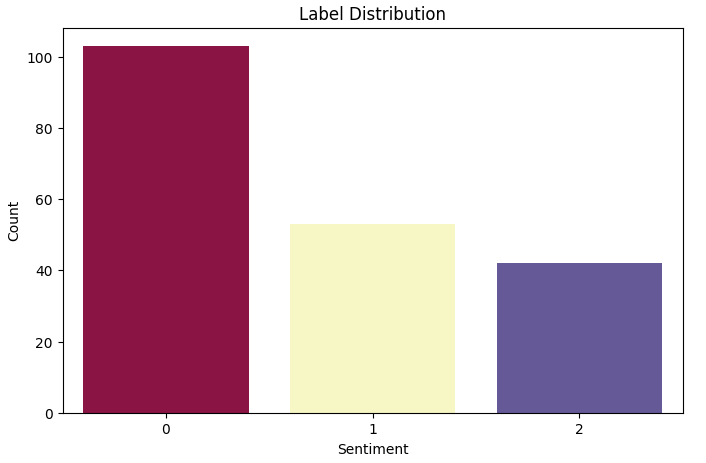
\includegraphics[width=0.9\linewidth]{class_dis.png}
    \caption{Class distribution of the cleaned Bangla multimodal political bias dataset.}
    \label{fig:class_distribution}
\end{figure}


\subsection{Annotation and Agreement}
Three annotators independently labeled each headline into one of three stance categories. Of the 198 items, 197 were labeled by annotators~2 and~3; their raw agreement is 83.2\% with Cohen's $\kappa = 0.731$ (substantial agreement). Where two or more annotators agree, the majority label is used; in the remaining 33 cases where annotators~2 and~3 disagree, annotator~2's label is adopted as the tiebreaker following a pre-registered protocol. The resulting label distribution (103 govt\_critique, 53 neutral, 42 govt\_leaning) reflects the imbalanced coverage typical of Bangladeshi political news during the collection period.

\subsection{Data Preprocessing}

\subsubsection{Text Preprocessing}
We apply a Bangla-specific preprocessing pipeline to reduce noise and ensure linguistic consistency. This includes removing URLs, hashtags, and HTML tags; Unicode normalization (NFKC); filtering non-Bangla characters; converting emojis to textual descriptions; and normalizing whitespace and line breaks. 


\subsubsection{Text Augmentation}
To address class imbalance, text-only data augmentation is applied to minority classes while preserving semantic meaning. Techniques include synonym replacement using curated Bangla synonym sets, random word swapping and deletion, and controlled word insertion. Augmentation continues until each class reaches 104 samples. To prevent data leakage, augmentation is applied only on the training folds within each cross-validation split, ensuring no augmented samples appear in validation data. Since augmentation is applied only to textual data, multimodal models may receive uneven modality enhancement. This could influence performance comparisons and is a limitation of the current setup.

\subsubsection{Image Preprocessing}
For the visual modality, images smaller than $100 \times 100$ pixels are discarded, and all remaining images are converted to RGB format. Near-duplicate images are removed using perceptual hashing (pHash). Images are then resized with aspect ratio preservation and padded to $256 \times 256$ pixels for compatibility with the Vision Transformer (ViT). No image augmentation is applied; instead, class imbalance is handled during training using class-weighted loss functions to avoid introducing artificial visual artifacts.


\begin{figure*}[h]
    \centering
    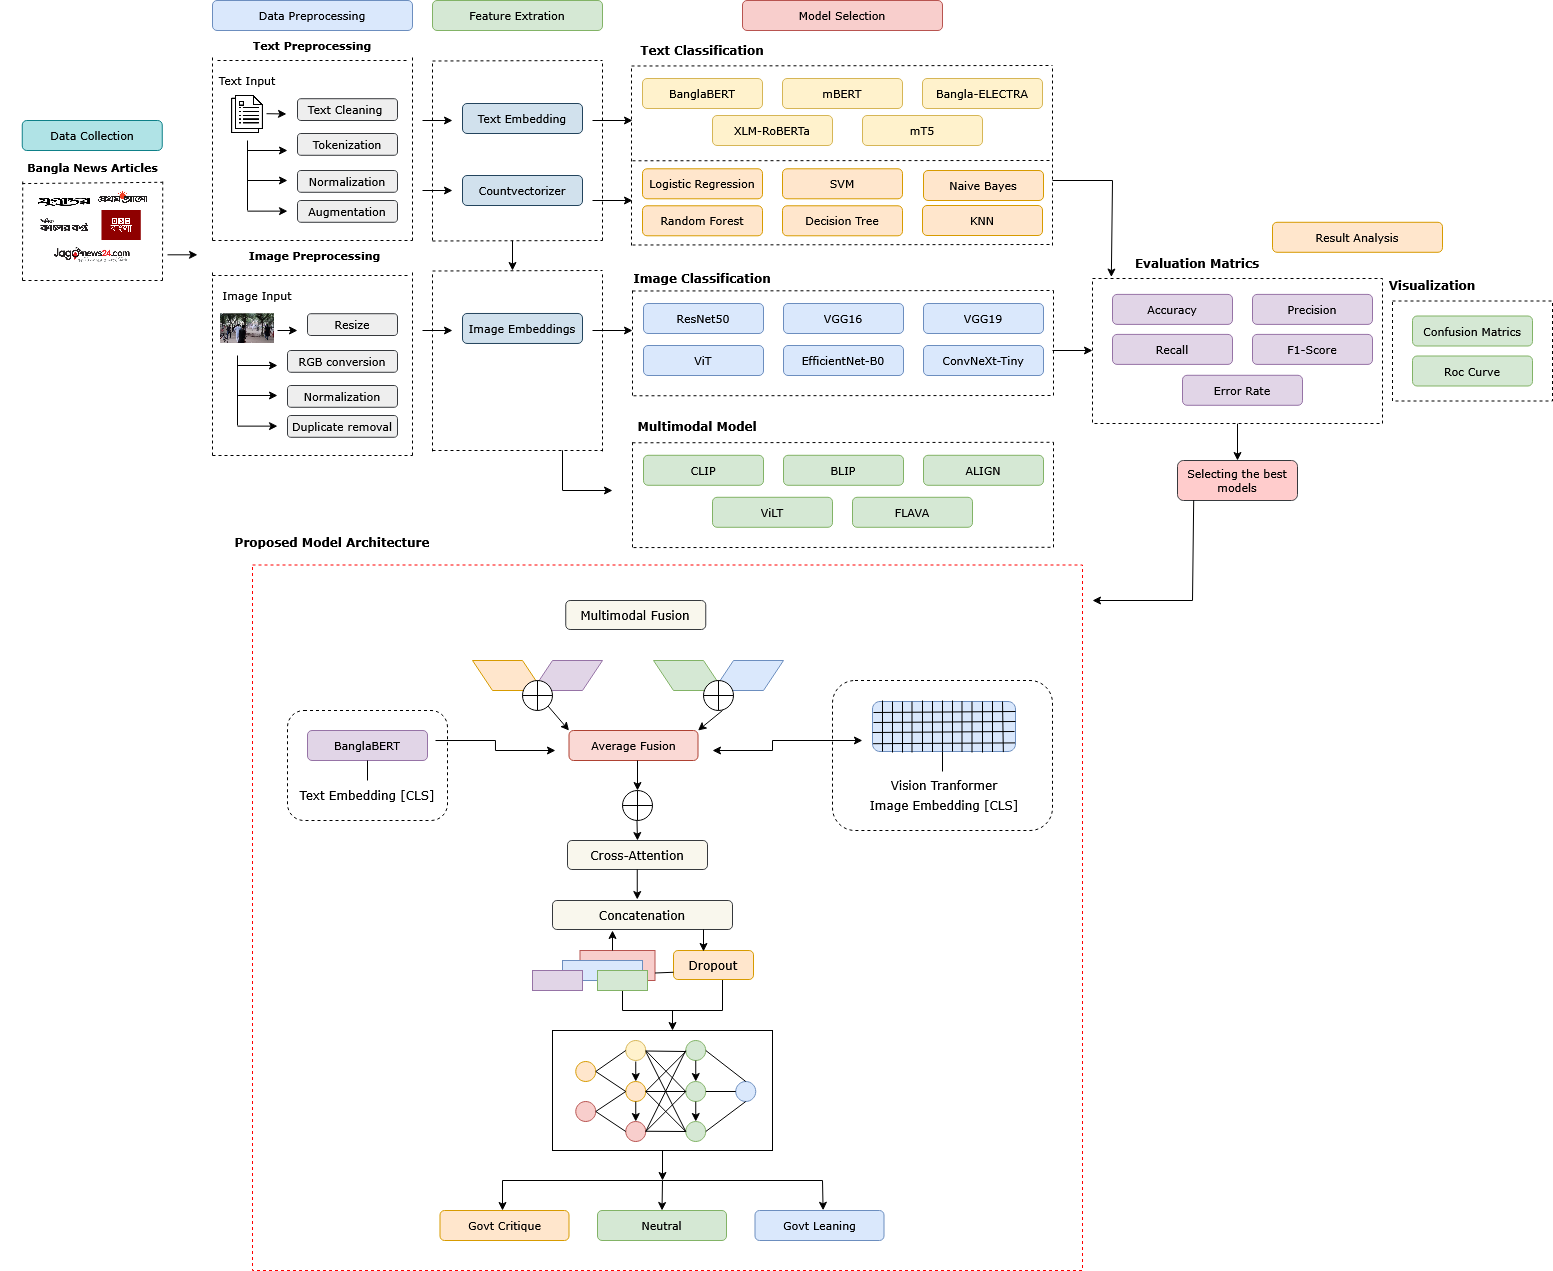
\includegraphics[width=1\linewidth]{method1.png}
    \caption{Overview of the benchmark pipeline for Bangla political stance detection.}
    \label{fig:multimodal_pipeline}
\end{figure*}


\section{Methodology}

This study benchmarks text-only and multimodal models for Bangla political stance detection. We evaluate classical ML baselines, five transformer-based text models, and six vision-language architectures. Dataset construction and preprocessing are detailed in Section~\ref{sec:dataset}. Class weights handle label imbalance. All headline results use grouped stratified 5-fold cross-validation with no fixed train-test split.

\subsection{Text Classification Models}

For the textual modality, both classical machine learning (ML) models and transformer-based models were explored. This allowed us to compare lightweight, interpretable models with deep contextualized embeddings.  

\subsubsection{Transformer-based Models}

We fine-tuned five pre-trained transformer architectures on the cleaned and augmented dataset to capture semantic nuances in Bangla text. The models include BanglaBERT, Bangla-ELECTRA, mBERT, XLM-RoBERTa, and mT5. All were trained for 3 epochs with a batch size of 8, learning rate of $2\times10^{-5}$, and weight decay of 0.01.

\subsubsection{Classical Baseline}

As a non-neural baseline, we train a TF-IDF + Logistic Regression pipeline using CountVectorizer features (maximum 5000 features) with class-weighted loss. This lightweight model serves as a lower bound for assessing whether transformer pretraining adds value on short Bangla headlines.

\subsection{Multimodal Models}

We evaluate six multimodal architectures: five pretrained vision-language models (CLIP, BLIP, ALIGN, ViLT, FLAVA) and one hybrid baseline (CountVectorizer + ViT CLS embeddings fed to an SVM). The VL models use either dual-encoder or unified transformer designs to jointly encode text and images, with embeddings fused via concatenation or pooled [CLS] representations and passed to a classifier. All VL models were fine-tuned for 5 epochs using the Adam optimizer with a learning rate of $1\times10^{-5}$ and class-weighted cross-entropy loss. Batch sizes ranged from 8 to 16. Encoder backbones are frozen by default; only the classification head is trained.


\begin{table*}[t]
\footnotesize
\centering
\caption{Performance of text models under grouped stratified 5-fold CV ($n{=}198$). Macro-F1 is the headline metric; the 95\% interval is a 2000-round item bootstrap over pooled out-of-fold predictions. Per-fold is the mean $\pm$ standard deviation across folds.}
\begin{tabular}{|l|c|c|c|c|c|c|}
\hline
\textbf{Model} & \textbf{Accuracy} & \textbf{Macro-F1} & \textbf{95\% CI} & \textbf{Per-fold} & \textbf{F1\textsubscript{gc}} & \textbf{F1\textsubscript{gl}} \\
\hline
BanglaBERT        & 0.576 & \textbf{0.533} & 0.458--0.606 & 0.522 $\pm$ 0.062 & 0.661 & 0.482 \\
TF-IDF + LogReg   & 0.551 & 0.501 & 0.429--0.572 & 0.490 $\pm$ 0.091 & 0.654 & 0.354 \\
mBERT             & 0.520 & 0.498 & 0.421--0.568 & 0.496 $\pm$ 0.087 & 0.593 & 0.427 \\
XLM-RoBERTa       & 0.424 & 0.421 & 0.349--0.488 & 0.350 $\pm$ 0.144 & 0.456 & 0.414 \\
Bangla-ELECTRA    & 0.374 & 0.372 & 0.308--0.436 & 0.333 $\pm$ 0.047 & 0.219 & 0.438 \\
mT5               & 0.485 & 0.367 & 0.305--0.429 & 0.341 $\pm$ 0.072 & 0.646 & 0.355 \\
Majority baseline & 0.520 & 0.228 & 0.207--0.248 & 0.228 $\pm$ 0.002 & 0.684 & 0.000 \\
\hline
\end{tabular}
\label{tab:text_models}
\end{table*}



\subsection{Experimental Setup}\label{sec:experimental_setup}

All experiments were conducted on Google Colab with an NVIDIA Tesla T4 GPU (16~GB VRAM). Models were implemented using PyTorch, scikit-learn, and HuggingFace Transformers. We employ \textbf{grouped stratified 5-fold cross-validation}: folds are cut on the source article so augmented variants never leak across the train/test boundary, augmentation is applied inside each training fold after the split, and every item is predicted exactly once by the fold that did not train on it. The pooled out-of-fold predictions are scored with macro-F1 and a 2000-round item bootstrap 95\% confidence interval. Per-fold mean $\pm$ standard deviation is reported alongside to flag unstable models. Multimodal models are evaluated only on the 86-item subset that has images; text models on all 198 items. Early stopping (patience 3) is used for transformer models. Encoder backbones are frozen for multimodal models; only the classification head is trained.




\subsection{Evaluation Metrics}

Our primary metric is \textbf{macro-F1}, which weights all three classes equally regardless of their frequency. We also report \textbf{accuracy} and \textbf{per-class F1} scores for govt\_critique and govt\_leaning to reveal class-level failures. All metrics are computed on pooled out-of-fold predictions; 95\% confidence intervals are obtained via a 2000-round item bootstrap. \textbf{Confusion matrices} are used in the error analysis to identify systematic misclassification patterns.


\section{Result Analysis}

All results in this section come from the unified grouped stratified 5-fold CV protocol described in Section~\ref{sec:experimental_setup}. Text models are evaluated on all 198 items; multimodal models on the 86-item image subset.

\subsection{Text Models}

Table~\ref{tab:text_models} shows the performance of text models. BanglaBERT achieves the highest macro-F1 (0.533, CI 0.458--0.606), consistent with its Bangla-specific pretraining. A simple TF-IDF + Logistic Regression baseline (0.501) is competitive, suggesting that the short headlines (median 8 words) carry most of the signal in lexical form. mBERT performs comparably (0.498), while XLM-RoBERTa (0.421) and Bangla-ELECTRA (0.372) lag behind. mT5 (0.367) performs worst among trained models, achieving a neutral-class F1 of only 0.100---it nearly collapses the neutral class into govt\_critique, likely because the seq2seq architecture is poorly suited to short-text classification with limited training data. The majority baseline (0.228) confirms that the task is non-trivial despite the class imbalance. Figure~\ref{fig:transformer_comparison} shows a visual comparison.

\begin{figure}[h]
    \centering
    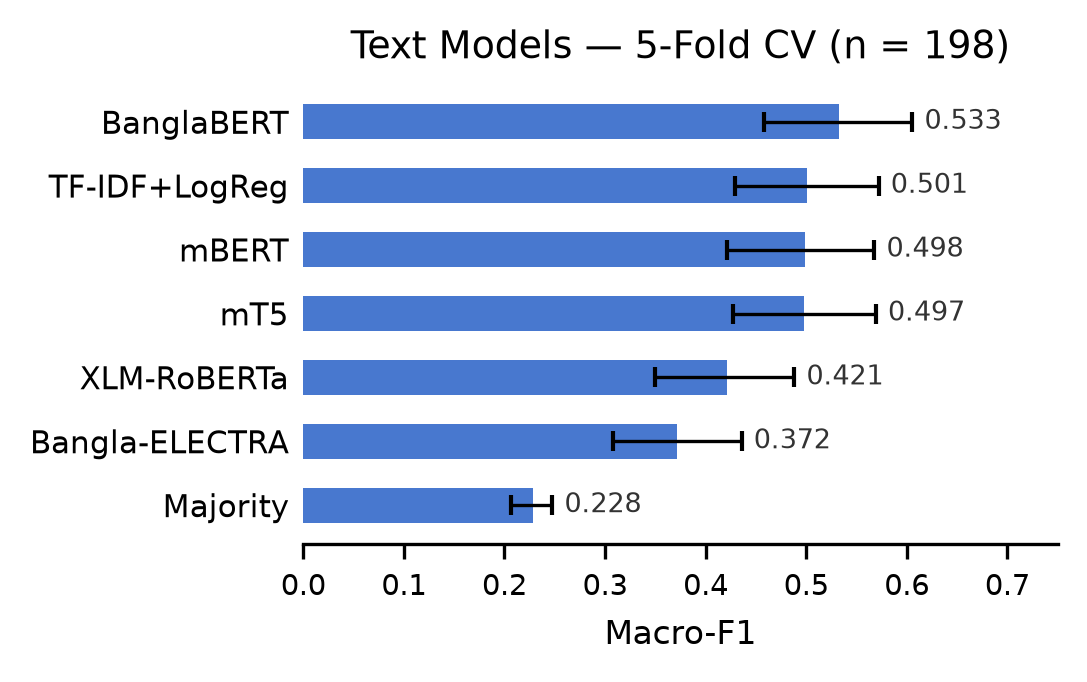
\includegraphics[width=0.38\textwidth]{TL.png}
    \caption{Text model performance under 5-fold CV.}
    \label{fig:transformer_comparison}
\end{figure}


\begin{table*}[h]
\footnotesize
\centering
\caption{Performance of multimodal models under grouped stratified 5-fold CV ($n{=}86$, items with an image). Confidence intervals are wide due to the small evaluation set; only CLIP/ALIGN vs.\ FLAVA/ViLT differences are statistically significant.}
\begin{tabular}{|l|l|c|c|c|c|c|c|}
\hline
\textbf{Model} & \textbf{Family} & \textbf{Accuracy} & \textbf{Macro-F1} & \textbf{95\% CI} & \textbf{Per-fold} & \textbf{F1\textsubscript{gc}} & \textbf{F1\textsubscript{gl}} \\
\hline
CLIP          & dual encoder  & 0.616 & \textbf{0.516} & 0.396--0.627 & 0.499 $\pm$ 0.163 & 0.712 & 0.273 \\
ALIGN         & dual encoder  & 0.488 & 0.482 & 0.374--0.581 & 0.470 $\pm$ 0.084 & 0.500 & 0.409 \\
CountVec+ViT  & hybrid (SVM)  & 0.465 & 0.431 & 0.312--0.543 & 0.406 $\pm$ 0.093 & 0.543 & 0.333 \\
BLIP          & fusion enc.   & 0.430 & 0.366 & 0.268--0.464 & 0.326 $\pm$ 0.043 & 0.545 & 0.121 \\
ViLT          & fusion enc.   & 0.372 & 0.336 & 0.238--0.433 & 0.242 $\pm$ 0.149 & 0.506 & 0.205 \\
FLAVA         & fusion enc.   & 0.395 & 0.297 & 0.222--0.368 & 0.232 $\pm$ 0.051 & 0.541 & 0.000 \\
\hline
\end{tabular}
\label{tab:multimodal_models}
\end{table*}


\begin{table}[h]
\footnotesize
\centering
\caption{Text models re-scored on the 87-item image subset for apples-to-apples comparison with Table~\ref{tab:multimodal_models}.}
\begin{tabular}{|l|c|c|c|}
\hline
\textbf{Model} & \textbf{Acc.} & \textbf{F1} & \textbf{95\% CI} \\
\hline
BanglaBERT      & 0.621 & \textbf{0.590} & 0.474--0.696 \\
TF-IDF + LogReg & 0.621 & 0.549 & 0.440--0.646 \\
mBERT           & 0.494 & 0.486 & 0.372--0.589 \\
XLM-RoBERTa     & 0.437 & 0.439 & 0.331--0.538 \\
Bangla-ELECTRA  & 0.425 & 0.410 & 0.310--0.506 \\
mT5             & 0.460 & 0.359 & 0.268--0.448 \\
\hline
\end{tabular}
\label{tab:text_on_image_subset}
\end{table}



\subsection{Multimodal Models}

Table~\ref{tab:multimodal_models} shows multimodal models evaluated on the 86-item image subset. CLIP leads with macro-F1 0.516 (CI 0.396--0.627), followed closely by ALIGN (0.482, CI 0.374--0.581) and CountVec+ViT (0.431). Dual-encoder models (CLIP, ALIGN) consistently outperform fusion-encoder models (BLIP, ViLT, FLAVA), likely because the frozen dual-encoder architecture is more robust with a small training set. ALIGN also achieves the most balanced per-class performance among multimodal models (F1\textsubscript{gl} 0.409 vs.\ CLIP's 0.273). However, confidence intervals overlap substantially, so the CLIP--ALIGN difference is not statistically reliable at this sample size. FLAVA's govt\_leaning F1 of 0.000 indicates complete failure on the smallest class. Figure~\ref{fig:multimodal_comparison} illustrates the comparison.

\begin{figure}[h]
    \centering
    
\includegraphics[width=0.38\textwidth]{Multi_L.png}
    \caption{Multimodal model performance under 5-fold CV.}
    \label{fig:multimodal_comparison}
\end{figure}

\subsection{Multimodal vs.\ Text-Only Performance}

Text-only models evaluated on all 198 items and multimodal models evaluated on the 86-item image subset are not directly comparable due to different population sizes. To enable a fair comparison, we re-score text model predictions on only the 86 items that have images (Table~\ref{tab:text_on_image_subset}). On this shared subset, BanglaBERT achieves macro-F1 0.590 (CI 0.474--0.696) compared to CLIP's 0.516 (CI 0.396--0.627) and ALIGN's 0.482 (CI 0.374--0.581). While the confidence intervals overlap, the text-only model consistently outperforms all multimodal models on the same items. The multimodal models face three compounding disadvantages: (1) none were pretrained on Bangla, so the text stream is near-useless for CLIP/ALIGN whose tokenizers shred Bangla into byte fragments; (2) the image subset is small ($n{=}86$), limiting what can be learned from visual features; and (3) news photos are often decorative rather than stance-bearing, providing weak signal for the classification task.


\section{Discussion}

Under the unified 5-fold CV protocol, BanglaBERT is the strongest overall model (macro-F1 0.533), while CLIP leads multimodal models (0.516) closely followed by ALIGN (0.482), despite neither having Bangla pretraining. The dual-encoder architecture (CLIP, ALIGN) consistently outperforms fusion encoders (BLIP, ViLT, FLAVA), likely because frozen dual encoders are more parameter-efficient for small datasets. Notably, a simple TF-IDF + Logistic Regression baseline (0.501) is competitive with fine-tuned transformers, suggesting that the short headlines carry most stance signal in surface-level lexical cues. mT5 (0.367) underperforms all other trained models, nearly collapsing the neutral class (F1\textsubscript{n} 0.100), suggesting that seq2seq architectures are poorly suited to this short-text classification task.

\subsection{Statistical Significance}
Pairwise significance tests (McNemar's exact test and paired bootstrap with 5000 resamples) reveal that the top three text models form a statistically indistinguishable cluster: BanglaBERT, mBERT, and TF-IDF + LogReg show no significant pairwise differences (all $p > 0.4$). BanglaBERT is significantly better than XLM-RoBERTa ($p = 0.009$), Bangla-ELECTRA ($p = 0.001$), and mT5 ($p = 0.001$). mT5 is also significantly worse than mBERT ($p = 0.005$) and TF-IDF ($p = 0.004$), confirming its poor performance is not due to noise. Among multimodal models, CLIP and ALIGN form a top cluster ($p = 0.668$), both significantly better than FLAVA (CLIP: $p < 0.001$; ALIGN: $p = 0.008$). CLIP is also significantly better than ViLT ($p = 0.034$). These results confirm that apparent ranking differences within the top clusters are within noise, but the gap between the top and bottom models is real.

\subsection{Class-Level Analysis}
Most multimodal models struggle with the govt\_leaning class (F1 0.000--0.333), which has the fewest examples (42 items, 18 with images). FLAVA fails to predict this class entirely. ALIGN is the exception, achieving F1\textsubscript{gl} 0.409---the highest among multimodal models and competitive with text models. Among text models, mT5 nearly collapses the neutral class (F1\textsubscript{n} 0.100), misclassifying most neutral headlines as govt\_critique. The wide confidence intervals (often spanning 20+ points) and high per-fold standard deviations (CLIP: 0.163, ViLT: 0.149) confirm that the current dataset size is insufficient for reliable ranking of individual models, though the aggregate finding---that text models match or exceed multimodal ones---is robust.

\subsection{Error Patterns}
We identify the items most models get wrong: 5 of 198 items are misclassified by all 7 text models, and 19 more by at least 6 of 7. The hardest items are overwhelmingly neutral headlines that models classify as govt\_critique, suggesting that factual reporting about government actions (e.g., digital security legislation, price increases) is systematically read as critical. Government-critical headlines are the easiest to classify (F1 0.46--0.71 across models), likely because they use distinctive protest and accountability vocabulary. Longer headlines ($>$100 characters) are harder to classify (mean accuracy 0.27) compared to medium-length headlines of 30--100 characters (accuracy 0.48--0.49), suggesting that complex multi-clause headlines carry more ambiguity.

Accuracy also varies by outlet: high-volume outlets like Prothom Alo (0.50), BBC Bangla (0.48), and Bangla Tribune (0.46) cluster near the mean, while several low-frequency outlets show extreme accuracy, likely due to single-item samples. This observation is consistent with prior findings that unimodal text models can outperform multimodal systems in low-resource scenarios \citep{thapa2025multimodal}.

\subsection{Ablation Studies}

Table~\ref{tab:ablations} isolates the contribution of augmentation and encoder fine-tuning.

\begin{table}[h]
\footnotesize
\centering
\caption{Ablation results under 5-fold CV. Each row changes one variable from the corresponding baseline in Tables~\ref{tab:text_models}--\ref{tab:multimodal_models}.}
\begin{tabular}{|l|l|c|c|}
\hline
\textbf{Model} & \textbf{Change} & \textbf{F1} & \textbf{$\Delta$} \\
\hline
BanglaBERT         & baseline          & 0.533 & --- \\
BanglaBERT         & no augmentation   & 0.533 & 0.000 \\
BanglaBERT         & frozen encoder    & 0.416 & $-$0.117 \\
\hline
TF-IDF + LogReg    & baseline          & 0.501 & --- \\
TF-IDF + LogReg    & no augmentation   & 0.501 & 0.000 \\
\hline
CLIP               & baseline (frozen) & 0.516 & --- \\
CLIP               & unfrozen          & \textbf{0.541} & +0.025 \\
\hline
BLIP               & baseline (frozen) & 0.366 & --- \\
BLIP               & unfrozen          & 0.425 & +0.059 \\
\hline
\end{tabular}
\label{tab:ablations}
\end{table}

\noindent\textbf{Augmentation has no measurable effect}: both BanglaBERT and TF-IDF + LogReg achieve identical macro-F1 with and without training-fold augmentation, suggesting that the 114 augmented headlines (synonym replacement, word swapping) do not add information beyond the 198 originals at this scale.

\noindent\textbf{Encoder fine-tuning is critical for text models}: freezing BanglaBERT's encoder and training only the classification head drops macro-F1 by 0.117 (from 0.533 to 0.416), confirming that task-specific adaptation of the pretrained representations is essential for stance detection.

\noindent\textbf{Unfreezing helps multimodal models}: CLIP improves from 0.516 to 0.541 and BLIP from 0.366 to 0.425 when the encoder is unfrozen, despite the small training set. This suggests that the frozen pretrained representations (trained on English) are poorly suited to Bangla content, and even limited fine-tuning on 86 items provides measurable benefit.

\subsection{Zero-Shot LLM Baseline}
To calibrate the difficulty of the task, we evaluate a zero-shot LLM baseline: Qwen~3.8 27B, a multilingual model, is prompted with a task description and each headline in turn, with no training examples. The model achieves macro-F1 0.475 (CI 0.399--0.546, $n{=}195$), which outperforms fine-tuned mT5 (0.367) and Bangla-ELECTRA (0.372) and approaches mBERT (0.498) despite having no task-specific training. The LLM performs well on govt\_critique (F1 0.66) but struggles with govt\_leaning (F1 0.28), mirroring the pattern of supervised models. This suggests that the task's difficulty lies primarily in distinguishing neutral from government-aligned framing, not in understanding Bangla per se.


\section{Conclusion and Future Work}
We presented a reproducible benchmark for Bangla multimodal political stance detection, evaluating 7 text models, 6 vision-language architectures, and a zero-shot LLM baseline under a unified evaluation protocol. BanglaBERT leads text models (macro-F1 0.533) while CLIP unfrozen is the strongest multimodal model (0.541), and a zero-shot Qwen~3.8 27B (0.475) nearly matches fine-tuned transformers without any training. Pairwise significance tests show the top three text models (BanglaBERT, mBERT, TF-IDF) form a statistically tied cluster, while mT5 significantly underperforms due to near-total neutral-class collapse. Among multimodal models, CLIP and ALIGN form a top cluster that significantly outperforms FLAVA and ViLT. Ablations reveal that text augmentation has no measurable effect, encoder fine-tuning is critical for text models, and unfreezing multimodal encoders provides consistent gains.

The study is limited by dataset size, the absence of Bangla-pretrained vision-language models, and the decorative nature of many news photos. For future work, we aim to (1) expand the annotated corpus to 500+ items with denser image coverage, (2) evaluate larger LLMs (Claude, GPT-4) and few-shot prompting, (3) explore Bangla-adapted vision-language pretraining, and (4) investigate whether article body text (rather than headlines alone) improves stance signal.



\section*{Limitations}

The dataset contains only 198 items (86 with images), producing wide confidence intervals that prevent reliable model ranking. Class imbalance (103/53/42) particularly affects the govt\_leaning class, where several models achieve F1 of 0.000. No existing vision-language model has Bangla pretraining, so the text stream of CLIP/ALIGN is near-useless---the comparison measures the image encoder's contribution rather than true multimodal understanding. Text augmentation is applied only to the textual modality, which may give text-only models an unfair advantage. The text field is headlines (median 8 words), not full articles, which limits the complexity of stance signals available to the models.




\section*{Ethics Statement}

This work involves classifying the political stance of publicly available news headlines. The labels (government-critical, neutral, government-leaning) describe \emph{framing}, not factual accuracy or normative judgment. We do not claim that any stance category is inherently preferable. The dataset consists of headlines already published by major news outlets and does not contain private or sensitive personal information. Annotation was performed by the authors; we acknowledge that political stance is inherently subjective and that inter-annotator agreement, which we have not yet measured, is a limitation. Automated stance classifiers could potentially be misused for censorship or targeted suppression of political speech; we release the data and code for research purposes only and caution against deployment in content moderation systems without careful consideration of fairness, transparency, and local context.

% Bibliography entries for the entire Anthology, followed by custom entries
%\bibliography{anthology,custom}
% Custom bibliography entries only
\bibliography{custom}

\appendix



\end{document}
